\section{The Verification Test}
\label{sec:verify}

Given a specification polynomial $f$, and a circuit $C$, the
verification test is formulated as presented in
\cite{lv:tcad2013}. The circuit is modeled by a set of multivariate
polynomials $F=\{f_1,\dots,f_s\}$ in the ring $R=\Fkk[x_1,\dots,x_n]$
for the given data-path (operand) size $k$, where $x_1,\dots,x_n$
denote the nets (signals) in the circuit. As the circuit comprises
Boolean logic gates, they are modeled as polynomials in $\F_2 \subset
\Fkk$:

\begin{equation}
\label{bool2poly}
\begin{split}
z ~ =  ~ \neg a ~ \rightarrow ~ z+a+1 & \pmod 2  \\
z ~ =  ~ a \wedge b ~ \rightarrow ~ z+a \cdot b & \pmod 2\\
z ~ =  ~ a \vee b ~ \rightarrow ~ z+a+b+a \cdot b & \pmod 2 \\
z ~ =  ~ a \oplus b ~ \rightarrow ~ z+a+b & \pmod 2 
\end{split}
\end{equation}

The set of polynomials $F$ generates an ideal, which we denote by $J =
\langle F\rangle$. When $C$ correctly implements $f$, then $f$ agrees
with every evaluation of all the nets in $C$. In other words, $f$
vanishes on $V(J)$, or equivalently $f \in I(V(J))$. The Strong
Nullstellensatz in finite fields (Thm. \ref{thm:strong-ns}) tells us
that $I(V(J)) = J + J_0$, where $J_0 = \langle x_i^q-x_i:
i=1,\dots,n\rangle$. Thus, the verification test can be formulated as
ideal membership testing of $f$ in $J+J_0$ using \Grobner bases: to
check if $f\xrightarrow{GB(J+J_0)}_+0$?

The \Grobner basis computation $GB(J+J_0)$ exhibits high
complexity, as it is shown to be bounded by
$q^{O(n)}$ \cite{gao:qe-gf-gb}. In \cite{wienand:cav08}
\cite{lv:tcad2013}, the authors showed that the expensive \Grobner
basis computation can be avoided altogether for this verification
test. It was shown that for any arbitrary combinational circuit, a
specialized term order can be derived by analyzing the topology of the
given circuit. Imposition of this term order on $R$ renders the set of
polynomials $F=\{f_1,\dots,f_s\}$ itself a \Grobner basis. Based on
Buchberger's product criteria, their approach exploits the fact
that {\it when the leading terms of all polynomials in $F$ are
  relatively prime, then $F$ already constitutes a \Grobner basis.}

\begin{Definition}
\label{def:rtto}
Let $C$ be an arbitrary combinational
circuit described by a set of polynomials $F=\{f_1,\dots,f_s\}$ with
variables $\{x_1,\dots,x_n\}$. Starting from the primary outputs,
perform a reverse topological traversal of $C$ and order the variables
such that $x_i>x_j$ if $x_i$ appears earlier in the reverse
topological order. Impose a {\it lex} term order $>$ to
represent each gate as a polynomial $f_i$, s.t. $f_i = x_i +
tail(f_i)$. Then the set $F=\{f_1, \dots, f_s\}$
forms a Gr\"obner basis, as $lt(f_i)=x_i$ and $lt(f_j)=x_j$ for
$i\neq j$ are relatively prime. This term order $>$ is called the {\bf
  Reverse Topological Term   Order (RTTO)}.  
\end{Definition}


Our formulations also contain $k$-bit word-level variables
corresponding to the input and output word-level operands. These
variables can also be accommodated in RTTO $>$ by imposing a lex term
order with variable order {\it Output word $>$ input words $>$
  bit-level variables ordered reverse topologically}.  In
\cite{lv:tcad2013}, the authors analyzed the effect of such a term
order further on ideal generators that include the vanishing
polynomials. Let $X_{PI} \subset \{x_1,\dots,x_n\}$  be the primary
input variables of the circuit. Let $F_0^{PI}=\{x_i^2-x_i:x_i\in
X_{PI}\}$ denote the set of bit-level vanishing polynomials in primary
inputs. We state the following result from \cite{lv:tcad2013}, which
we utilize in our formulation. 


\begin{Proposition}\label{prop:rtto}
(Corollary 6.1 in \cite{lv:tcad2013}) Using RTTO $>$ to represent the
  polynomials in $R$, the set $F\cup F_{0}^{PI}$ constitutes a
  \Grobner basis of $J+J_0$.  
\end{Proposition}

The benefit of using RTTO $>$ is that the verification test can be
performed solely by way of polynomial division
$f\xrightarrow{F,F_{0}^{PI}}_+r$, and by checking whether or not $r=0$?
If $r=0$, then $C$ implements $f$. Otherwise when $r\neq 0$, there
exists a bug in the design. Moreover, RTTO $>$ ensures that when
$r\neq 0$, $r$ comprises only primary input variables $X_{PI}$. Any
assignment to $X_{PI}$ that makes $r\neq 0$ generates a
counter-example that can be used for debugging. 

We use the verification setup under RTTO $>$ (i.e. Def. \ref{def:rtto}
and Prop. \ref{prop:rtto}) to rectify the circuit. Our approach begins
when the verification test detects the presence of a bug in the
design, i.e. $f\xrightarrow{F,F_{0}^{PI}}_+r$ with $r\neq 0$. 
In the sequel, we will use the circuit shown in
Fig. \ref{fig:mas_both} as a running example to demonstrate our
approach to debugging and rectification. The circuit is a modified
version of a Mastrovito multiplier \cite{mastro:1989}, where extra
redundant logic was first added in the circuit, and then a bug was
introduced in the redundant logic. 

%% \begin{figure*}[ht]
%%     \begin{center}
%%     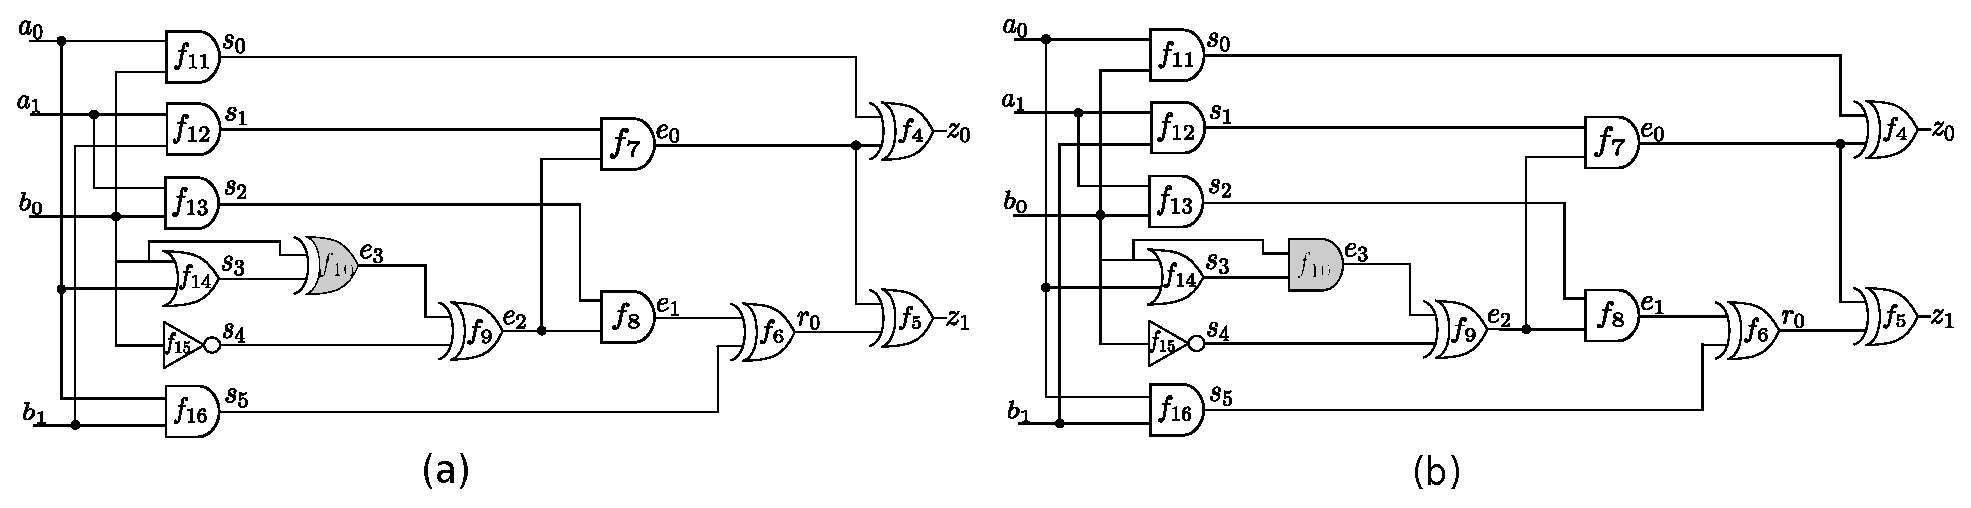
\includegraphics[scale = 0.5]{mas_both.eps}
%%     \end{center}
%% %    \vspace{-4ex}
%%     \caption{Design verification of a 2-bit finite-field multiplier:
%%       (a) Buggy design, with incorrect gate implemented implemented at
%%     net $e_3$. (b) A correct implementation.}
%%     \label{fig:mas_both}
%%     \vspace{-2ex}

%% \end{figure*}

\vspace{2ex}

\begin{figure}[hbt]
    \begin{center}
    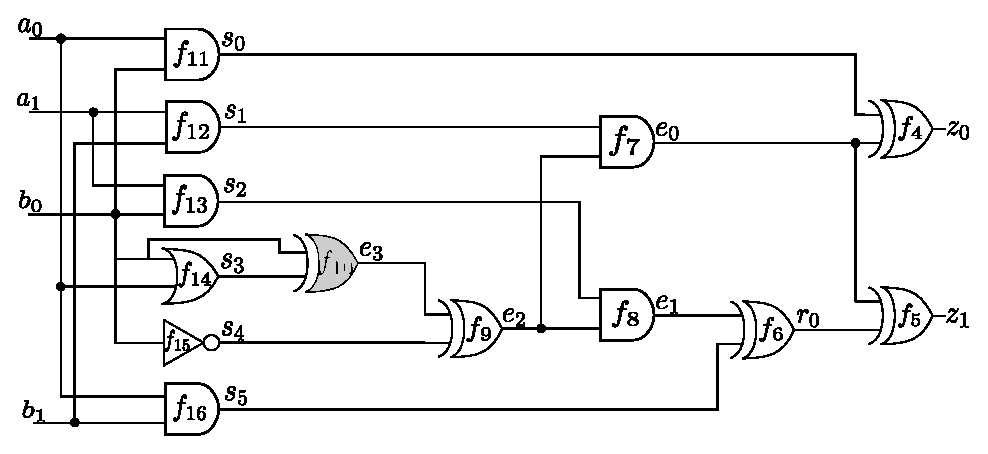
\includegraphics[scale = 0.5]{mas_red_bug.eps}
    \end{center}
%    \vspace{-4ex}
    \caption{\small Design verification of a 2-bit finite-field
      multiplier. The circuit is buggy, with the bug introduced at
    net $e_3$. A correct implementation includes an AND gate at $e_3$,
    which is replaced by an XOR gate to introduce a bug.}
    \label{fig:mas_both}
    \vspace{-3ex}
\end{figure}

\begin{Example}
  \label{ex:1}
We perform verification of the design of a 2-bit finite field
multiplier in $\F_4$, where the output $Z$ is to be computed as
$A\cdot B$, where 
$Z = \{z_1,z_0\}, A=\{a_1,a_0\}, B=\{b_1,b_0\}$ are the given 2-bit
operands. Assume further that $P(X) = X^2+X+1$ is the irreducible
polynomial used to construct $\F_4 = \F_2[X]\pmod{ P(X)}$, with
$P(\alpha)=0$.

The implemented circuit $C$ is given as shown in
Fig. \ref{fig:mas_both}. Denote polynomial $f: Z + A\cdot B$ as the
design specification. For the verification test, we perform a reverse
topological traversal of the circuit to derive RTTO $>$, i.e. a {\it
  lex} term order with variable order:
$\{Z\}>\{A>B\}>\{z_0>z_1\}>\{r_0\}>\{e_0>e_1\}>\{e_2\}>\{e_3\}>\{s_0>s_1>s_2>s_3>s_4>s_5\}>\{a_0>a_1>b_0>b_1\}$\\ 
The polynomials describing the circuit are given as:
% \begin{equation*}
% \begin{split}
% f_1:s_0 + a_0*b_0;  &  f_5:r_0 + s_1 + s_2; & f_8:A + a_0 + a_1*\al; \\
% f_2:s_3 + \mathcal{F}(a_1,b_1);  &  f_6:z_0 + s_0 + s_3; & f_9:B + b_0 + b_1*\al;\\
% f_3:s_2 + a_1*b_0;  &  f_7:z_1 + r_0 + s_3; & f_{10}:Z + z_0 + z_1*\al;\\
% f_4:s_1 + a_0*b_1;
% \end{split}
% \begin{equation}

\vspace{-0.1in}

{\small\begin{flalign*}
f_1:Z + z_0 +\al z_1;  &\quad f_9:e_2 + e_3 + s_4;   \\
f_2:A + a_0 +\al a_1;  &\quad f_{10}:e_3 + b_0 + s_3; \\
f_3:B + b_0 +\al b_1;  &\quad f_{11}:s_0 + a_0b_0; \\
f_4:z_0 + s_0 + e_0;    &\quad f_{12}:s_1 + a_1b_1; \\
f_5:z_1 + e_0 + r_0;    &\quad f_{13}:s_2 + a_1b_0; \\
f_6:r_0 + e_1 + s_5;    &\quad f_{14}:s_3 + a_0 + b_0 + a_0b_0; \\
f_7:e_0 + s_1e_2;       &\quad f_{15}:s_4 + b_0 + 1;\\
f_8:e_1 + s_2e_2;               &\quad f_{16}:s_5 + a_0b_1; 
\end{flalign*}}

\vspace{-0.1in}
Then $F = \{f_1,\dots,f_{16}\}$, $F_0^{PI} = \{a_0^2-a_0, a_1^2-a_1,
b_0^2-b_0, b_1^2-b_1\}$, and $F\cup F_{0}^{PI}$ constitutes a \Grobner
basis of $J+J_0$. Computing $f\xrightarrow{F,F_{0}^{PI}}_+r$ gives $r
=
(\alpha+1)a_0a_1b_1b_0+(\alpha+1)a_0a_1b_1+(\alpha+1)a_1b_1b_0+(\alpha)a_1b_0$. Since 
$r\neq 0$, the presence of a bug in the design is detected. Our
objective now is to identify a net where rectification can be
performed, and then to subsequently identify a rectification function. 
\end{Example}

%% Note that a similar approach can be employed when equivalence
%% verification is to be performed between two gate level circuits
%% $C_1,C_2$. As in a gate-level miter, the inputs of $C_1,C_2$ are
%% connected together. Let the output words computed by $C_1, C_2$ be
%% $Z_{1}, Z_{2}$, respectively. RTTO $>$ can be computed for both
%% circuits to represent $C_1,C_2$ using the set of polynomials
%% $F_1,F_2$, respectively.  Denote the polynomial $f=Z_{1}-Z_{2}$. Then
%% the two circuits implement the same function iff
%% $f\xrightarrow{F_1,F_2,F_{0}^{PI}}_+0$, as $F_1\cup F_2 \cup
%% F_{0}^{PI}$ still constitutes a \Grobner basis. 
